\documentclass[12pt]{article}

\usepackage{graphicx}
\usepackage[margin=1.0in]{geometry}
\usepackage{amsmath}
\usepackage{cases}
\usepackage{amsfonts}
\usepackage{amssymb}
\usepackage{grffile}
\usepackage{setspace}

\setlength\parindent{0pt}

\author{Xiaohui Chen \\EID: xc2388}
\title{M 362K Pre-Class Work for 1/29}

\begin{document}
\maketitle
\begin{spacing}{2.0}

\section*{2-35}
From the question we know that $Pr(call-dad)=0.01$, $Pr(is- dad|call-dad)=0.90$, $Pr(is-dad|not-call-dad)=0.05$

$Pr(call-dad|is-dad)=\frac{Pr(call-dad\cap is-dad)}{Pr(is-dad)}= \frac{Pr(is-dad|call-dad)*Pr(call-dad)}{Pr(is-dad)}=$

$\frac{Pr(is-dad|call-dad)*Pr(call-dad)}{Pr(is-dad|call-dad)* Pr(call-dad)+ Pr(is-dad|not-call-dad)*Pr(not-call-dad)} =\frac{0.9*0.01}{0.9*0.01+0.05*0.99}=0.1538$

\section*{2-38}
\begin{figure}
  \centering
  % Requires \usepackage{graphicx}
  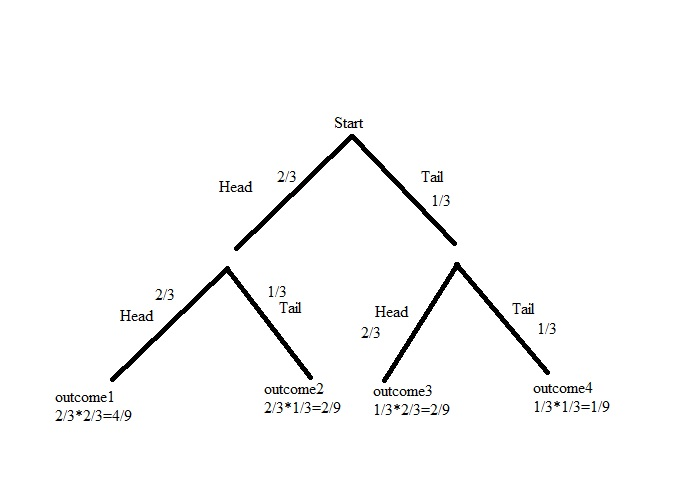
\includegraphics[width=5.5in]{tree}\\
  \caption{Tree Diagram for 2-38}\label{tree}
\end{figure}

All the probabilities are shown in Figure \ref{tree}

\section*{2-40}
From the question we know that $Pr(B|A)=\frac{12}{51}$

Since $Pr(B)=\frac{13}{52}=\frac{1}{4}\ne Pr(B|A)$, A and B are dependent

\section*{2-53}
Assume the number of blue balls in the second urn is x

Since the two events in both urns are independent, we can know that $Pr(same-color)=Pr(both-red)+Pr(both-blue)= \frac{4}{10}*\frac{16}{x+16}+\frac{6}{10}*\frac{x}{x+16}=0.44$

$\therefore x=4$

There are 4 blue balls in the second urn. The answer is (A)

\end{spacing}
\end{document}